\documentclass[12pt,addpoints]{exam}

\usepackage{geometry}
\geometry{letterpaper, margin = 1in}

\usepackage{graphicx}

\usepackage{amsmath}

\usepackage{mathptmx}

\title{\vspace{-1in}Final Exam}
\author{College Algebra}
\date{}

\pagestyle{empty}

\begin{document}

\maketitle

\flushright{\textbf{Name:} \underline{\hspace{2in}}}

\begin{questions}
	\question[5] If Mary Johnson weighed 145 lbs. in 1986 and weighed 190 lbs. in 2007. Find the rate of change in her weight between 1986 and 2007. Include the units. Round your answer to two decimal places.
	\vspace{\fill}   

	\question[5] Does the data in the following table determine a linear function or an exponential function? Explain your answer.
	
\begin{tabular}{|c|c|c|c|c|}
	\hline
	$x$ & 2 & 4 & 6 & 8 \\ \hline
	$y$ & 8 & 128 & 2048 & 32768 \\ \hline
\end{tabular}
	\vspace{\fill}

	\question The following graph shows the average American houseful debt $h$ has a function of the date $d$.
	
	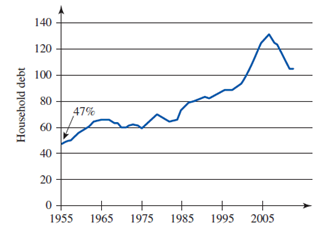
\includegraphics[width=3in]{final_exam_1.png}
	
	\begin{parts}
		\part[2] Explain the meaning of $h(1975)$ in practical terms. \vspace{0.5in}
		
		\part[1] Use the graph to find $h(1975)$. Write the units. \vspace{0.25in}
		
		\part[1] The graph reaches a maximum value. Estimate the maximum value. \vspace{0.25in}
		
		\part[1] Estimate the year in which the maximum value occured. \vspace{0.25in}
	\end{parts}

	\newpage

	\question[5] Use the crossing-graphs method to solve the given equation. Round your answer to three decimal places.
	$$ \frac{15}{2 + 3^x} = x$$ \vspace{1in}
	
	\question Data about recenent federal defense spending are given in the accompanying \textit{Statistical Abstract of the United States} table. Here $t$ denotes time, in years since 1990, and $D$ denotes federal defensee spending, in billions of dollars.
	
	\begin{tabular}{|c|c|c|c|c|c|} \hline
	$t$ years since 1990 & 0 & 5 & 10 & 15 & 20 \\ \hline
	$D$ Federal spending & 328.4 & 210.0 & 341.5 & 565.5 & 843.8 \\ \hline
	\end{tabular}

	\begin{parts}
		\part[2] Calculate the average rate of change in defense spending from 1990 to 1995. Include the units. \vspace{\fill}
		\part[2] Use your answer from part (a) to estimate $D(3)$. Show your work. \vspace{\fill}
		
		\part[1] Explain in practical terms what the value you calculated in part (b) means. \vspace{\fill}
	\end{parts}

	\newpage
	
	\question You have decided to open a t-shirt printint business. A silk-screening machine is available for \$1,400 and bulk t-shirts cost \$1.90 each.
	\begin{parts}
		\part[3] Using function notation, construct a model that expresses the total cost as a function of the number of t-shirts printed. Use $n$ for the number of t-shirts printed and $C$ for the total cost in dollars. \vspace{\fill}
		
		\part[2] Determine the number of t-shirts you can initially print if you have \$2,000 to get started. \vspace{\fill}
	\end{parts}
	
	\question The following table shows the Untied States Gross National Product (GNP), in tillions of dollars, during a specific year $t$. Here, $t=0$ is 1995.

	\begin{tabular}{|c|c|c|c|c|c|} \hline
	$t = \text{year}$ & 3 & 4 & 5 & 6 & 7 \\ \hline
	$G = \text{GNP}$ & 7.78 & 8.31 & 8.85 & 9.11 & 9.44 \\ \hline
	\end{tabular}
	\begin{parts}
		\part[2 \half] Determine the linear regression line for the data set. Write the equation in terms of $t$ and $G$. Round the parameters to three decimal places. \vspace{\fill}
		\part[2 \half] Use the regression equation to find the number of years it will take fo rthe GNP to be 16 trillions dollars. Round to three decimal places. \vspace{\fill}
	\end{parts}
	
	\newpage
	
	\question[5] Solve the system of linear equations using matrices.
	\begin{align*}
		6x - y + 5z &= -28 \\
		4x + 2y &= 10 \\
		5x + 6z &= -23
	\end{align*} \vspace{\fill}

	\question In 2007, there were about 3.8 gigawatts of solar photovoltaic installations. From 2007 through 2014, the industry showed exponential growth, with a yearly growth factor of 1.45.
	\begin{parts}
		\part[2] Make an exponential model that shows the photovoltaic installations $P$, in gigawatts, at a time $t$ years after 2007. \vspace{\fill}
		\part[2] Use this model to estimate the photovoltaic installations (in gigawatts) in 2011. Round your answer to two decimal places. \vspace{\fill}
		\part[1] Explain in practical terms the meaning of $P(5)$ in this problem. Do not calculate the value.\vspace{\fill}
	\end{parts}

	\newpage
	
	\question A report tells us that in 2009, there were 870 gray wolves in Idaho, but that the population declined by 17\% that year. For the purposes of this problem, we assume that this 17\% annual rate of decrease continues.
	\begin{parts}
		\part[2 \half] Find an exponential model that gives the wolf population $W$ as a function of time $t$ in years since 2009. \vspace{\fill}
		
		\part[2 \half] It is expected that the wolf population cannot recover if there are fewer than 30 individuales. How long must this rate of decline continue for the wolf population to reach 30? Round your answer to two decimal places. \vspace{\fill}
	\end{parts}

	\question The table below shows the amount, in grams, of a substance as it decays over time in days.
	\begin{tabular}{|c|c|c|c|c|} \hline
		$t = \text{Days}$ 3 & 6 & 9 & 12 \\ \hline
		$A = \text{amount}$ 15.35 & 9.43 & 5.8 & 3.56 \\ \hline
	\end{tabular}
	\begin{parts}
		\part[3] Determine the equation of the exponential regression curve that best fits the data set. Round your answer to three decimal places. \vspace{\fill}
		\part[2] What is the decay factor? In practical terms explain what it means. \vspace{\fill}
	\end{parts}
	
	\newpage
	
	\question A regular-sized girls' basketball was bounced from a certain height. The following data was collected and rounded to the nearest hundredth. Time is in seconds.
	
	\begin{tabular}{|c|c|} \hline
	Time (t) & Height (ft) \\ \hline
	0.01 & 1.88 \\ \hline
	0.11 & 3.05 \\ \hline
	0.21 & 4.13 \\ \hline
	0.31 & 4.91 \\ \hline
	0.41 & 5.37 \\ \hline
	0.51 & 5.50 \\ \hline
	0.61 & 5.31 \\ \hline
	0.71 & 4.82 \\ \hline
	0.81 & 4.00 \\ \hline
	0.91 & 2.97 \\ \hline
	\end{tabular}
	\begin{parts}
		\part[2] Use regression to find a quadratic model for the data. Round the regression parameters to two decimal places. \vspace{0.5in}
		\part[3] Using the regression model found in part (a), when will the ball first be 3.28 feet off the ground? Write the equation that yo uuse to solve the problem. Round your answer to two decimal places. \vspace{\fill}
	\end{parts}
	
	\question[5] Use the quadratic formula $\left( x = \frac{-b \pm \sqrt{b^2 - 4 ac}}{2a} \right)$ to find the $x$-intercepts of the following function. Round your answer to two decimal places.
	$$y = x^2 + 3.58 x - 6$$ \vspace{\fill}
	
	\newpage
	
	\question[5] Solve the following question algebraically. Round your answer to two decimal places. Show your work.
	$$-4 \log(3x) = -15$$ \vspace{\fill}
	
	\question[5] Solve the following question algebraically. Round your answer to two decimal places. Show your work.
	$$5 e^{x+2} = 14$$ \vspace{\fill}
	
	\question[5] Find the inverse of the following function.
	$$ g(x) = \frac{6x+7}{5} $$ \vspace{\fill}
	
	\newpage
	
	\question[5] Given $f(x) = 2x^2 + 4$ and $g(x) = -3x$, calculate $f(g(x))$ and simplify. Show your work. \vspace{\fill}
	
	\bonusquestion The cost $C$ and the revenue $R$ for a brokerage firm depend on the number $t$ of transactions executed. (Both $C$ and $R$ are measured in dollars.) It costs \$730 per day to keep the office open, and brokers are paid an average of \$22 per transaction. Also, \$32 in fees are collected for each transaction.
	\begin{parts}
		\bonuspart[2] Find a formula that gives $C$ as a function of $t$. \vspace{\fill}
		\bonuspart[2] Find a formula that gives $R$ as a function of $t$. \vspace{\fill}
	\end{parts}
	
	\end{questions}
	
	\begin{center}
		\combinedgradetable[h][pages]
	\end{center}
	
\end{document}